% Options for packages loaded elsewhere
\PassOptionsToPackage{unicode}{hyperref}
\PassOptionsToPackage{hyphens}{url}
%
\documentclass[
  12pt,
  titlepage,
  draft]{ltjsarticle}
\usepackage{amsmath,amssymb}
\usepackage{lmodern}
\usepackage{iftex}
\ifPDFTeX
  \usepackage[T1]{fontenc}
  \usepackage[utf8]{inputenc}
  \usepackage{textcomp} % provide euro and other symbols
\else % if luatex or xetex
  \usepackage{unicode-math}
  \defaultfontfeatures{Scale=MatchLowercase}
  \defaultfontfeatures[\rmfamily]{Ligatures=TeX,Scale=1}
\fi
% Use upquote if available, for straight quotes in verbatim environments
\IfFileExists{upquote.sty}{\usepackage{upquote}}{}
\IfFileExists{microtype.sty}{% use microtype if available
  \usepackage[]{microtype}
  \UseMicrotypeSet[protrusion]{basicmath} % disable protrusion for tt fonts
}{}
\makeatletter
\@ifundefined{KOMAClassName}{% if non-KOMA class
  \IfFileExists{parskip.sty}{%
    \usepackage{parskip}
  }{% else
    \setlength{\parindent}{0pt}
    \setlength{\parskip}{6pt plus 2pt minus 1pt}}
}{% if KOMA class
  \KOMAoptions{parskip=half}}
\makeatother
\usepackage{xcolor}
\usepackage{color}
\usepackage{fancyvrb}
\newcommand{\VerbBar}{|}
\newcommand{\VERB}{\Verb[commandchars=\\\{\}]}
\DefineVerbatimEnvironment{Highlighting}{Verbatim}{commandchars=\\\{\}}
% Add ',fontsize=\small' for more characters per line
\newenvironment{Shaded}{}{}
\newcommand{\AlertTok}[1]{\textcolor[rgb]{1.00,0.00,0.00}{\textbf{#1}}}
\newcommand{\AnnotationTok}[1]{\textcolor[rgb]{0.38,0.63,0.69}{\textbf{\textit{#1}}}}
\newcommand{\AttributeTok}[1]{\textcolor[rgb]{0.49,0.56,0.16}{#1}}
\newcommand{\BaseNTok}[1]{\textcolor[rgb]{0.25,0.63,0.44}{#1}}
\newcommand{\BuiltInTok}[1]{\textcolor[rgb]{0.00,0.50,0.00}{#1}}
\newcommand{\CharTok}[1]{\textcolor[rgb]{0.25,0.44,0.63}{#1}}
\newcommand{\CommentTok}[1]{\textcolor[rgb]{0.38,0.63,0.69}{\textit{#1}}}
\newcommand{\CommentVarTok}[1]{\textcolor[rgb]{0.38,0.63,0.69}{\textbf{\textit{#1}}}}
\newcommand{\ConstantTok}[1]{\textcolor[rgb]{0.53,0.00,0.00}{#1}}
\newcommand{\ControlFlowTok}[1]{\textcolor[rgb]{0.00,0.44,0.13}{\textbf{#1}}}
\newcommand{\DataTypeTok}[1]{\textcolor[rgb]{0.56,0.13,0.00}{#1}}
\newcommand{\DecValTok}[1]{\textcolor[rgb]{0.25,0.63,0.44}{#1}}
\newcommand{\DocumentationTok}[1]{\textcolor[rgb]{0.73,0.13,0.13}{\textit{#1}}}
\newcommand{\ErrorTok}[1]{\textcolor[rgb]{1.00,0.00,0.00}{\textbf{#1}}}
\newcommand{\ExtensionTok}[1]{#1}
\newcommand{\FloatTok}[1]{\textcolor[rgb]{0.25,0.63,0.44}{#1}}
\newcommand{\FunctionTok}[1]{\textcolor[rgb]{0.02,0.16,0.49}{#1}}
\newcommand{\ImportTok}[1]{\textcolor[rgb]{0.00,0.50,0.00}{\textbf{#1}}}
\newcommand{\InformationTok}[1]{\textcolor[rgb]{0.38,0.63,0.69}{\textbf{\textit{#1}}}}
\newcommand{\KeywordTok}[1]{\textcolor[rgb]{0.00,0.44,0.13}{\textbf{#1}}}
\newcommand{\NormalTok}[1]{#1}
\newcommand{\OperatorTok}[1]{\textcolor[rgb]{0.40,0.40,0.40}{#1}}
\newcommand{\OtherTok}[1]{\textcolor[rgb]{0.00,0.44,0.13}{#1}}
\newcommand{\PreprocessorTok}[1]{\textcolor[rgb]{0.74,0.48,0.00}{#1}}
\newcommand{\RegionMarkerTok}[1]{#1}
\newcommand{\SpecialCharTok}[1]{\textcolor[rgb]{0.25,0.44,0.63}{#1}}
\newcommand{\SpecialStringTok}[1]{\textcolor[rgb]{0.73,0.40,0.53}{#1}}
\newcommand{\StringTok}[1]{\textcolor[rgb]{0.25,0.44,0.63}{#1}}
\newcommand{\VariableTok}[1]{\textcolor[rgb]{0.10,0.09,0.49}{#1}}
\newcommand{\VerbatimStringTok}[1]{\textcolor[rgb]{0.25,0.44,0.63}{#1}}
\newcommand{\WarningTok}[1]{\textcolor[rgb]{0.38,0.63,0.69}{\textbf{\textit{#1}}}}
\usepackage{longtable,booktabs,array}
\usepackage{calc} % for calculating minipage widths
% Correct order of tables after \paragraph or \subparagraph
\usepackage{etoolbox}
\makeatletter
\patchcmd\longtable{\par}{\if@noskipsec\mbox{}\fi\par}{}{}
\makeatother
% Allow footnotes in longtable head/foot
\IfFileExists{footnotehyper.sty}{\usepackage{footnotehyper}}{\usepackage{footnote}}
\makesavenoteenv{longtable}
\setlength{\emergencystretch}{3em} % prevent overfull lines
\providecommand{\tightlist}{%
  \setlength{\itemsep}{0pt}\setlength{\parskip}{0pt}}
\setcounter{secnumdepth}{5}
\usepackage{luatexja}
\usepackage[haranoaji]{luatexja-preset}
\usepackage{pagella-otf}
\usepackage{csquotes}
\usepackage{booktabs,siunitx,array,threeparttable}
\usepackage{tikz}
\usepackage{lipsum}
\makeatletter
\@ifpackageloaded{subfig}{}{\usepackage{subfig}}
\@ifpackageloaded{caption}{}{\usepackage{caption}}
\captionsetup[subfloat]{margin=0.5em}
\AtBeginDocument{%
\renewcommand*\figurename{Figure}
\renewcommand*\tablename{Table}
}
\AtBeginDocument{%
\renewcommand*\listfigurename{List of Figures}
\renewcommand*\listtablename{List of Tables}
}
\newcounter{pandoccrossref@subfigures@footnote@counter}
\newenvironment{pandoccrossrefsubfigures}{%
\setcounter{pandoccrossref@subfigures@footnote@counter}{0}
\begin{figure}\centering%
\gdef\global@pandoccrossref@subfigures@footnotes{}%
\DeclareRobustCommand{\footnote}[1]{\footnotemark%
\stepcounter{pandoccrossref@subfigures@footnote@counter}%
\ifx\global@pandoccrossref@subfigures@footnotes\empty%
\gdef\global@pandoccrossref@subfigures@footnotes{{##1}}%
\else%
\g@addto@macro\global@pandoccrossref@subfigures@footnotes{, {##1}}%
\fi}}%
{\end{figure}%
\addtocounter{footnote}{-\value{pandoccrossref@subfigures@footnote@counter}}
\@for\f:=\global@pandoccrossref@subfigures@footnotes\do{\stepcounter{footnote}\footnotetext{\f}}%
\gdef\global@pandoccrossref@subfigures@footnotes{}}
\@ifpackageloaded{float}{}{\usepackage{float}}
\floatstyle{ruled}
\@ifundefined{c@chapter}{\newfloat{codelisting}{h}{lop}}{\newfloat{codelisting}{h}{lop}[chapter]}
\floatname{codelisting}{Listing}
\newcommand*\listoflistings{\listof{codelisting}{List of Listings}}
\makeatother
\ifLuaTeX
  \usepackage{selnolig}  % disable illegal ligatures
\fi
\usepackage[style=apa,]{biblatex}
\addbibresource{bibliography.bib}
\IfFileExists{bookmark.sty}{\usepackage{bookmark}}{\usepackage{hyperref}}
\IfFileExists{xurl.sty}{\usepackage{xurl}}{} % add URL line breaks if available
\urlstyle{same} % disable monospaced font for URLs
\hypersetup{
  pdftitle={論文タイトル},
  pdfauthor={言文 花子},
  hidelinks,
  pdfcreator={LaTeX via pandoc}}

\title{論文タイトル}
\usepackage{etoolbox}
\makeatletter
\providecommand{\subtitle}[1]{% add subtitle to \maketitle
  \apptocmd{\@title}{\par {\large #1 \par}}{}{}
}
\makeatother
\subtitle{論文サブタイトル}
\author{言文 花子}
\date{}

\begin{document}
\maketitle
\begin{abstract}
論文の要旨\ldots 論文の要旨\ldots 論文の要旨\ldots 論文の要旨\ldots{}
論文の要旨\ldots 論文の要旨\ldots 論文の要旨\ldots 論文の要旨\ldots{}
論文の要旨\ldots 論文の要旨\ldots 論文の要旨\ldots 論文の要旨\ldots{}
論文の要旨\ldots 論文の要旨\ldots 論文の要旨\ldots 論文の要旨\ldots{}
論文の要旨\ldots 論文の要旨\ldots 論文の要旨\ldots 論文の要旨\ldots{}
論文の要旨\ldots 論文の要旨\ldots 論文の要旨\ldots 論文の要旨\ldots{}
論文の要旨\ldots 論文の要旨\ldots 論文の要旨\ldots 論文の要旨\ldots{}
\end{abstract}

{
\setcounter{tocdepth}{3}
\tableofcontents
}
\listoffigures
\listoftables
\newpage

\hypertarget{ux521dux3081ux306b}{%
\section{初めに}\label{ux521dux3081ux306b}}

\lipsum[1-2]

\begin{equation}\protect\hypertarget{eq:some_measure}{}{x = \lim_{inf}\alpha}\label{eq:some_measure}\end{equation}

As can be seen in eq.~\ref{eq:some_measure}, there is\ldots{}

Hello Hello Hello Hello Hello Hello Hello Hello Hello

日本語で論文を書く。\textbf{日本語で論文を書きたい。}
日本語で論文を書く。日本語で論文を書く。
日本語で論文を書く。日本語で論文を書く。
日本語で論文を書く。日本語で論文を書く。
日本語で論文を書く。日本語で論文を書く。
日本語で論文を書く。日本語で論文を書く。
日本語で論文を書く。日本語で論文を書く。
日本語で論文を書く。日本語で論文を書く。
日本語で論文を書く。日本語で論文を書く。
日本語で論文を書く。日本語で論文を書く。

我想用日语写一篇论文。我想用日语写一篇论文。
我想用日语写一篇论文。我想用日语写一篇论文。
我想用日语写一篇论文。我想用日语写一篇论文。
我想用日语写一篇论文。我想用日语写一篇论文。
我想用日语写一篇论文。我想用日语写一篇论文。
我想用日语写一篇论文。我想用日语写一篇论文。
我想用日语写一篇论文。我想用日语写一篇论文。
我想用日语写一篇论文。我想用日语写一篇论文。
我想用日语写一篇论文。我想用日语写一篇论文。

\begin{figure}
\centering
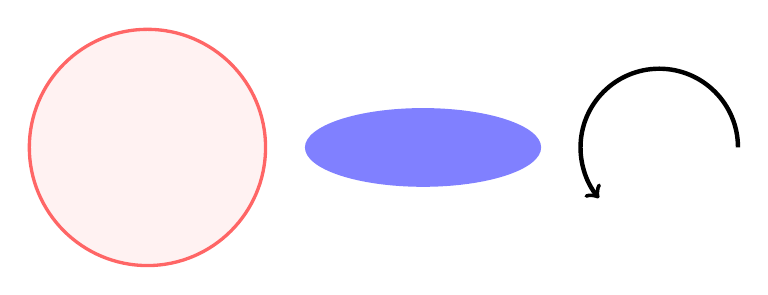
\begin{tikzpicture}
\filldraw[color=red!60, fill=red!5, very thick](-1,0) circle (1.5);
\fill[blue!50] (2.5,0) ellipse (1.5 and 0.5);
\draw[ultra thick, ->] (6.5,0) arc (0:220:1);
\end{tikzpicture}
\caption{図の例}
\end{figure}

\hypertarget{sec:previous_research}{%
\section{先行研究}\label{sec:previous_research}}

\lipsum[1-4]

\autocite{benjamin_reconstructing_2012,hodoscek_readability_2012,dubay_smart_2007,pitler_revisiting_2008,sato_automatic_2008,Sato2008}

\textcite{shibasaki_japanese_2010} によれば,\ldots{}

\hypertarget{tbl:my_table}{}
\begin{longtable}[]{@{}ll@{}}
\caption{\label{tbl:my_table}Demonstration of simple table
syntax.}\tabularnewline
\toprule()
\textbf{column1} & \textbf{column2} \\
\midrule()
\endfirsthead
\toprule()
\textbf{column1} & \textbf{column2} \\
\midrule()
\endhead
1 & 2 \\
3 & 4 \\
\bottomrule()
\end{longtable}

As we can see in tbl.~\ref{tbl:my_table}, this is \ldots{}

\hypertarget{ux30c7ux30fcux30bf}{%
\section{データ}\label{ux30c7ux30fcux30bf}}

sec.~\ref{sec:previous_research} に書いたように\ldots{}

\lipsum[1-4]

\hypertarget{ux30c7ux30fcux30bfux306eux8a73ux7d30}{%
\subsection{データの詳細}\label{ux30c7ux30fcux30bfux306eux8a73ux7d30}}

\begin{table}[!h]
\centering
\begin{threeparttable}
\caption{Valores de afinidad obtenidos para los ocho fármacos en \textit{Autodock Vina}}
\begin{tabular}{@{} l S[table-format=6.0] l S[table-format=5.0] cc @{}}
\toprule
{nº} & {CID Ligando} & {Nombre Ligando} & {Afinidad} & \multicolumn{2}{c@{}}{RMSD} \\
\cmidrule(l){5-6}
& & & {(Kcal/mol)\textsuperscript{2}} & {l.b.} & {u.b.}\\
\midrule
  1 & 234523 & LoremIpsum & 234   & 0 & 0 \\
  2 & 2345   & LoremIpsum & 2365  & 0 & 0 \\
  3 & 3453   & LoremIpsum & 45634 & 0 & 0 \\
  4 & 83452  & LoremIpsum & 2456  & 0 & 0 \\
\addlinespace
  5 & 210    & LoremIpsum & 245   & 0 & 0 \\
  6 & 3417   & LoremIpsum & 45634 & 0 & 0 \\
  7 & 4345   & LoremIpsum & 3456  & 0 & 0 \\
  8 & 4334   & LoremIpsum & 3456  & 0 & 0 \\
\bottomrule
\end{tabular}
\label{tab:version2}
\end{threeparttable}
\end{table}

\hypertarget{ux65b9ux6cd5}{%
\section{方法}\label{ux65b9ux6cd5}}

\lipsum[1-4]

\begin{Shaded}
\begin{Highlighting}[]
\ImportTok{import}\NormalTok{ spacy}

\NormalTok{nlp }\OperatorTok{=}\NormalTok{ spacy.load(}\StringTok{"ja\_ginza\_electra"}\NormalTok{)}

\ControlFlowTok{with} \BuiltInTok{open}\NormalTok{(}\StringTok{"corpus.txt"}\NormalTok{) }\ImportTok{as}\NormalTok{ f:}
\NormalTok{    text }\OperatorTok{=}\NormalTok{ f.read()}

\NormalTok{lemmas }\OperatorTok{=}\NormalTok{ [token.lemma\_ }\ControlFlowTok{for}\NormalTok{ token }\KeywordTok{in}\NormalTok{ nlp.pipe(text)]}
\end{Highlighting}
\end{Shaded}

\hypertarget{ux7d50ux679c}{%
\section{結果}\label{ux7d50ux679c}}

\lipsum[1-4]

\hypertarget{ux8003ux5bdf}{%
\section{考察}\label{ux8003ux5bdf}}

\lipsum[1-4]

\hypertarget{ux7d42ux308fux308aux306b}{%
\section{終わりに}\label{ux7d42ux308fux308aux306b}}

\lipsum[5-5]

\printbibliography

\end{document}
